% -------------------------------------------------------------------------------------------------
%
%  Skeleton for theses at the Institute of Robotics and Intelligent Systems
%
% -------------------------------------------------------------------------------------------------
%
% FILENAME:   thesis.tex
%
% ABSTRACT:   main file for theses
%
% USAGE:      compile with PDFLaTeX
%
% EXCEPTIONS: -
%
% HISTORY:    written by Sascha A. Stoeter <stoeter@iris.ethz.ch>, www.stoeter.com, 02.06.2004
%             modified by Martin Probst, 18.08.2004
% -------------------------------------------------------------------------------------------------

\documentclass[12pt,a4paper]{article}
\usepackage{iristhesis}

% -------------------------------------------------------------------------------------------------
% Add needed packages. Some generally useful packages are listed for
% your convenience.
% -------------------------------------------------------------------------------------------------
\usepackage{subfigure}                          % enable the use of subfigures
%\usepackage[bf]{caption}                       % must go after subfigure
\usepackage[thickspace,thinqspace]{SIunits}     %
\usepackage{natbib}
\usepackage{hyperref}

% enable Hyperlinks in pdf/ps Docs


% -------------------------------------------------------------------------------------------------
% Some handy definition to simplify future markup changes
% -------------------------------------------------------------------------------------------------
\providecommand{\eg}{e.g.}
\providecommand{\etal}{\textit{et al.}}
\providecommand{\ie}{i.e.}


% -------------------------------------------------------------------------------------------------
% Select type of thesis
% -------------------------------------------------------------------------------------------------
%\renewcommand{\iristhesistype}{Semester}
%\renewcommand{\iristhesistype}{Diploma}
\renewcommand{\iristhesistype}{Master}
%\renewcommand{\iristhesistype}{Ph.D.}

% -------------------------------------------------------------------------------------------------
% Set names
% -------------------------------------------------------------------------------------------------
\renewcommand{\irisauthor}{Theodore N. Koutros}
\renewcommand{\irisadviser}{Clark Teeple, George Chatzipirpiridis}


% -------------------------------------------------------------------------------------------------
% Beginning of the main document body
% -------------------------------------------------------------------------------------------------
\begin{document}

% include all Bib-items even if they're not cited in the text
%\nocite{*}
\bibliographystyle{ieeetr}
% This is the first part of the front matter. Pages appear unnumbered
% and the pages are not counted.

% Title page: set title and date preferably formatted according to
% ISO 8601
\iristitlepage{Optimizing the Functionality of a Soft-robotic Actuator}{2018-19}


% This is the second part of the front matter. Pages appear with
% lowercase roman numbering. The first page number is 'i'.
\pagenumbering{roman}

% Dedication (optional)
\newpage
%\thispagestyle{empty}
\markright{}
\vspace*{\stretch{1}}
\begin{center}
    To some special person
\end{center}
\vspace*{\stretch{2}}

% Preface (optional)
\markright{Preface}
\section*{Preface}

Thanks to whomever and other first words.


% Abstract must not be longer than one page per language. English and
% German abstracts are mandatory.
\addcontentsline{toc}{section}{\protect\numberline{}{Abstract}}
\markright{Abstract}
\section*{Abstract}

Short summary of thesis.

\addcontentsline{toc}{section}{\protect\numberline{}{Zusammenfassung}}
\markright{Zusammenfassung}
\section*{Zusammenfassung}

Kurzfassung der Arbeit.


% Table of contents
\newpage
\tableofcontents
\addtocontents{toc}{\vspace{.5\baselineskip}}

% List of tables
\newpage
\addcontentsline{toc}{section}{\protect\numberline{}{List of Tables}}
\listoftables

% List of figures
\newpage
\addcontentsline{toc}{section}{\protect\numberline{}{List of Figures}}
\listoffigures

% Glossary kind of chapters
\addcontentsline{toc}{section}{\protect\numberline{}{Notation}}
\addtocontents{toc}{\vspace{.5\baselineskip}}
\markright{Notation}
\section*{Notation}
\label{s:Notation}

Explanation of symbols.



% This is the main part of the thesis. Pages appear with arabic numbering.

\clearpage
\pagenumbering{arabic}

% Main body
\section{Introduction}
\label{s:Introduction}
This report will guide you through the work done in the past six months at the Harvard Micro-robotics Lab. 

Soft robotics are a developing field in  the world of automated devices. In most of the cases conventional robots are composed of rigid links  and supported by an algorithm based on the physical model to create predictable movements. These properties are very useful especially in industrial setups such as the automotive industry. With proper control repeatable tasks can be fulfilled with high precision and safety (using safeguards).  Soft-robots though,  are defined as having a reduced to low rigidity body and show flexibility and compliance with the environment and the objects they interact with. Stresses caused from any contact will first make the robot yield and comply before causing any significant damage to the target e.g., living organisms and humans. \cite{trivedi2008soft, rus2015design, polygerinos2017soft}. Therefore they can give a user a certain confidence when it comes to fulfilling a mission with low to null damage. Their rather simplified control adds to their usability, and a potential larger range of use cases. Without any wordplay, this feature makes them very flexible.

\subsection{Inspiration}
\label{s:Inspiration}
As humans we often want to mimic and reproduce phenomena we observe in nature. We especially focus on those we think will improve our lives and seek inspiration in all kinds of living creatures that surround us, from the deep seas to the rain-forests. 
Inspiration in soft-robotics is mainly biological and comes from animals like cephalopods (see Figure~\ref{f:Inspiration}), jellyfish or humans themselves. Even particular parts of the bodies are of specific interest such as elephant trunks (see Figure~\ref{f:Inspiration}\footnote{Pinterest: https://www.pinterest.ch/pin/345510602657383002/}) or the human tongue which are hydrostatic muscles. They rely on the incompressible property of water to actuate themselves. Through muscular cells and fibers they form elongated soft structures that are very adaptable (taking various shapes and positions). They can go through various elongations, bending and torsion modes. The octopus is a good example of a fully soft organism with no rigid skeleton. Composed of eight arms around a head, it is able to change itself to fit the environment and go through various holes and complicated mazes\footnote{National Georgraphic: https://youtu.be/SCAIedFgdY0}. Squids on the other hand have a few rigid cartilages supporting their body in an elongated nose cone-like shape allowing them to move fast in water.Though both are still molluscs (invertebrate). The same analogy can be done in soft robotics where different applications require a variety of compliance and stiffness properties thanks to inner or outer structures including links, plates or rods.

\begin{figure}[ht]
\centering
\subfigure[Pair of cuttlefish]{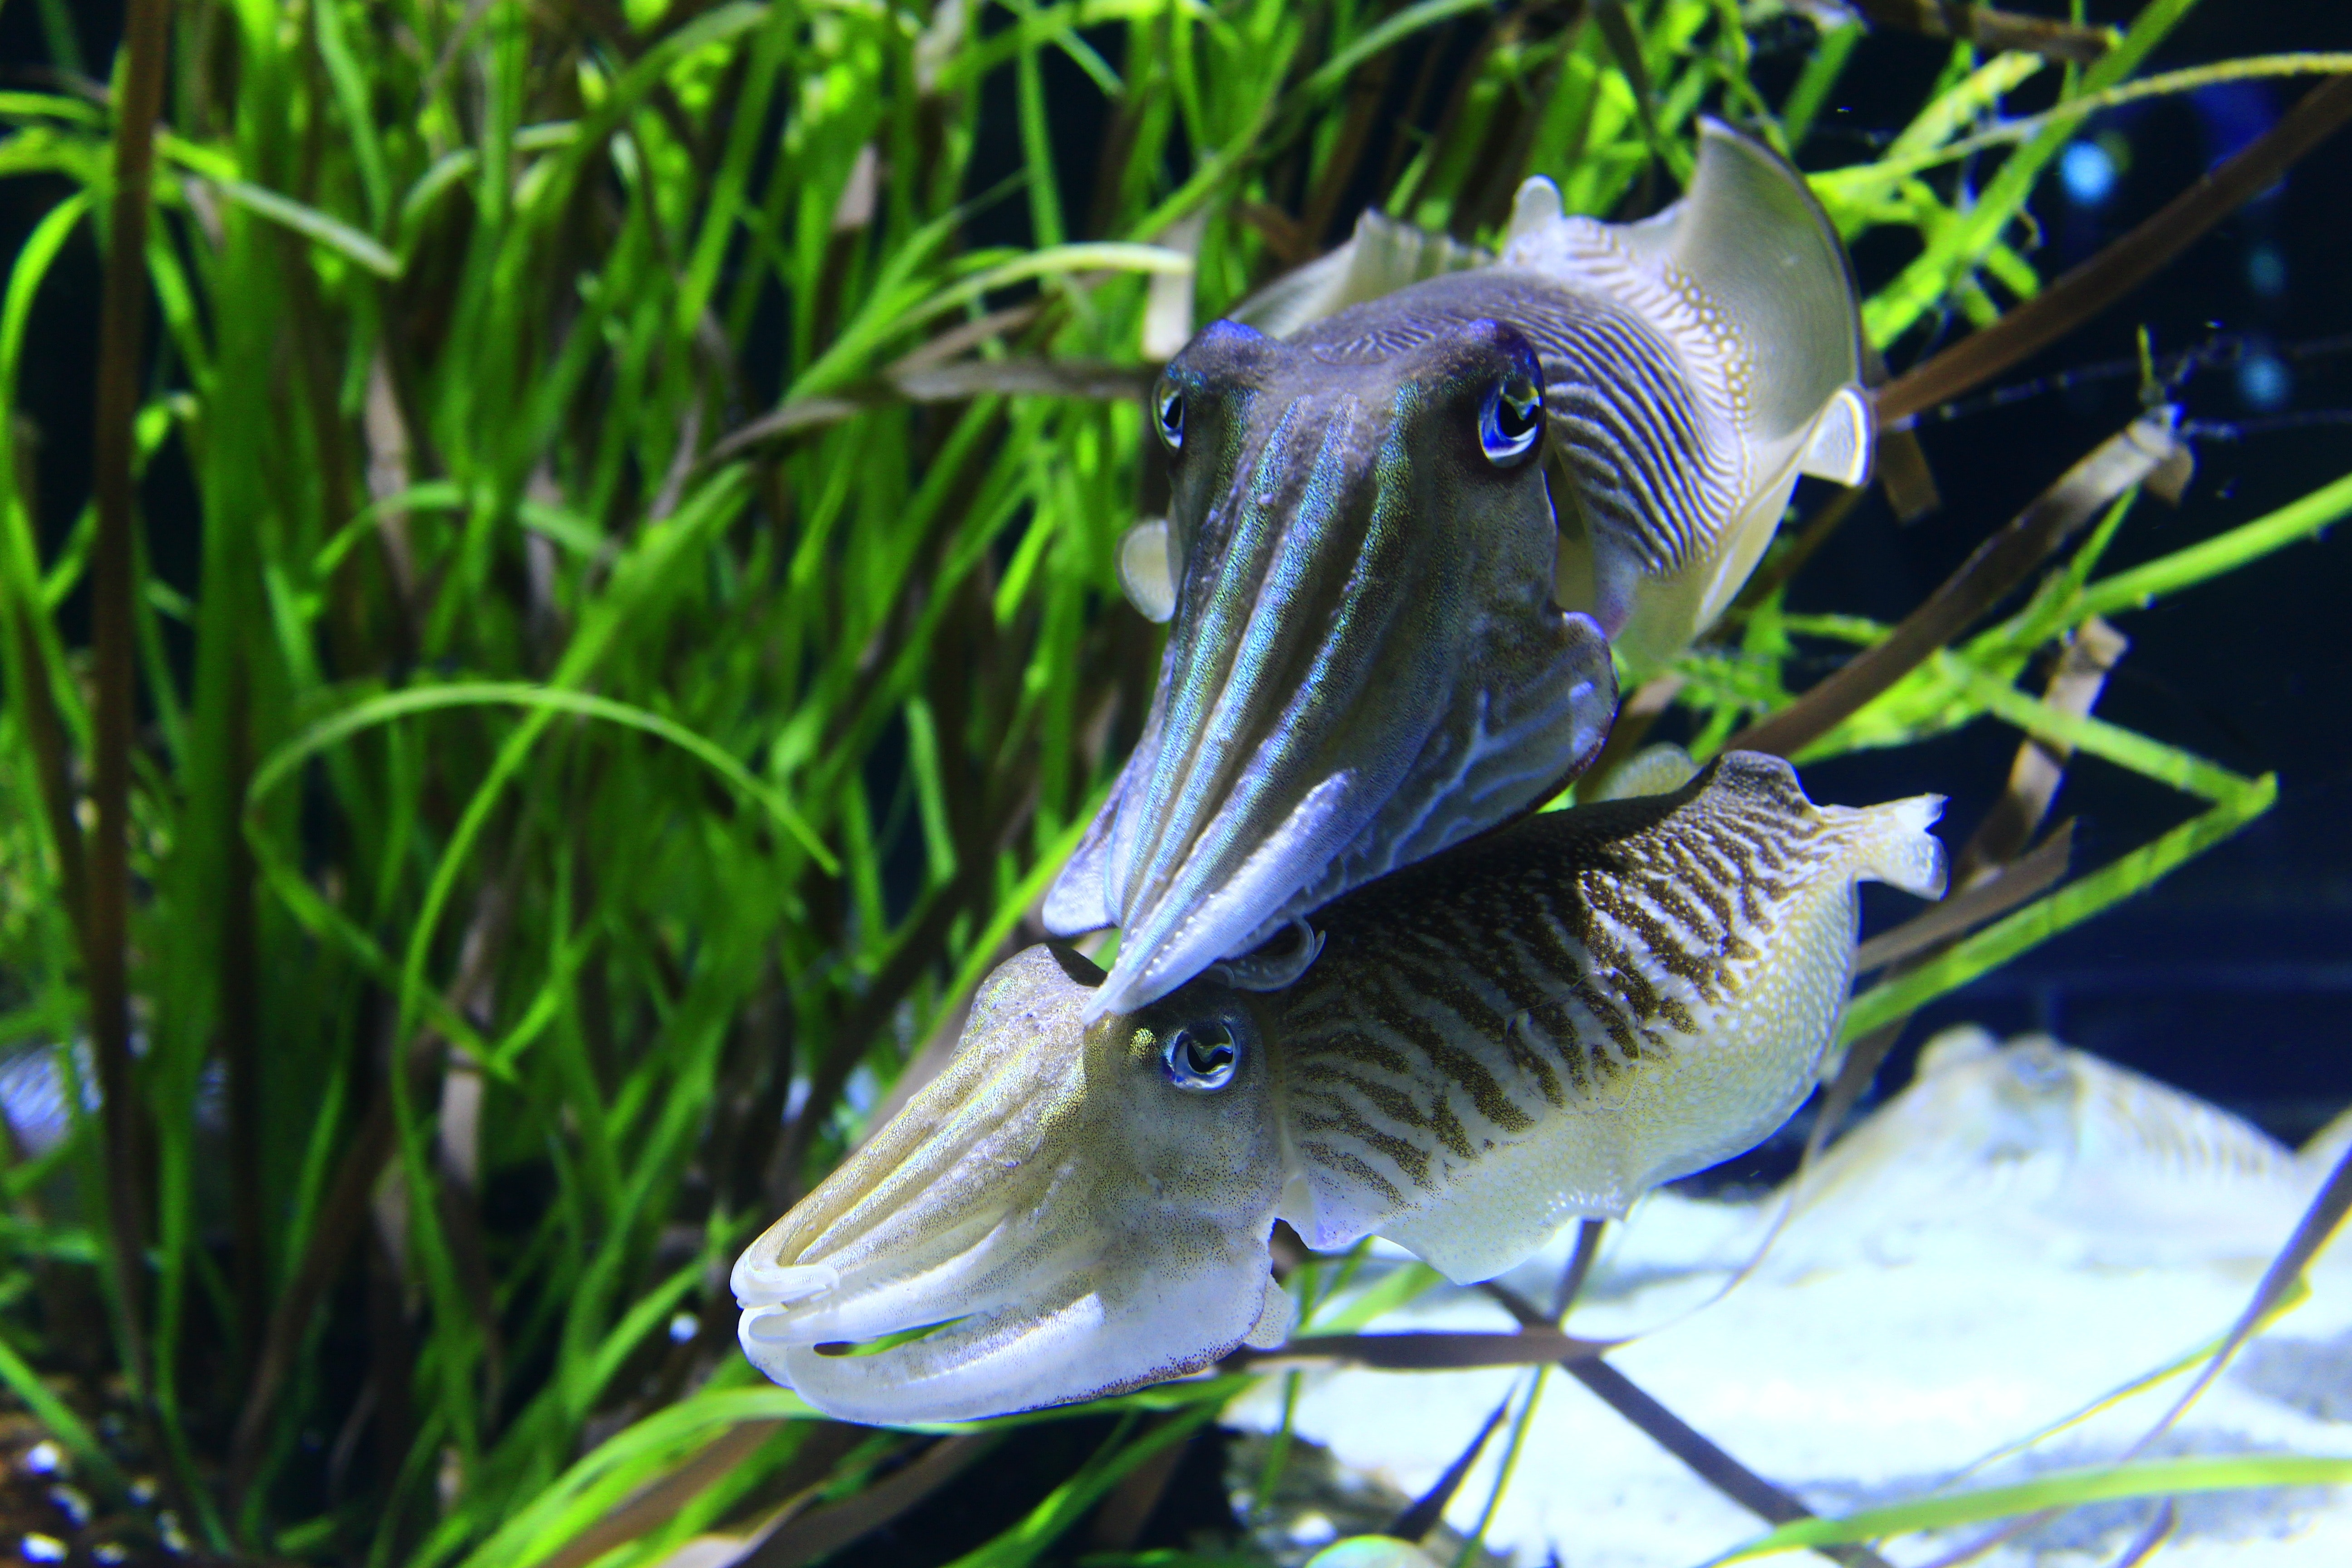
\includegraphics[height=50mm]{Images/cuttlefish.jpg}}\quad
\subfigure[Elephant trunk]{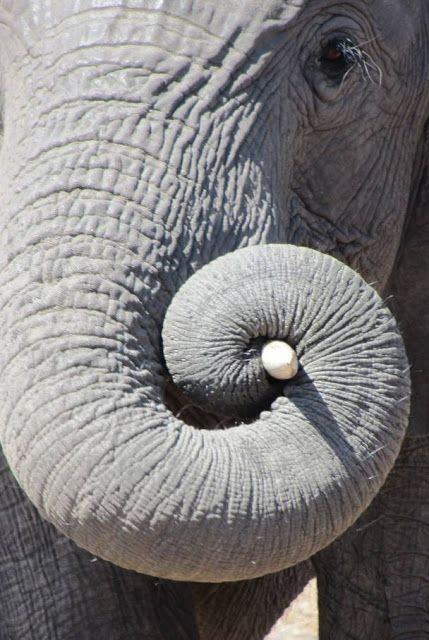
\includegraphics[height=50mm]{Images/elephant_trunk.jpg}}
\caption[Inspiration]{\label{f:Inspiration}(a) Cuttlefish are cephalopods with a rigid backbone.(b) A curled elephant trunk is a good example of a muscular hydrostat.}
\end{figure}


\subsection{Application}
\label{s:Application}
Soft robotic applications are very broad, the focus is , though,  mainly set on interactions with fragile and sensitive objects or living organisms (humans included). Even though common robots do perform very well (in medicine : da Vinci \footnote{da Vinci: https://www.intuitive.com/}), they are often very expensive and complex \cite{polygerinos2017soft}. Due to a similar impedance soft-robots reduce destructive contact forces allowing a safer manipulation. However this characteristic comes with a trade-off: the softer the robot the more difficult it is to manage its shape and  movements without reintroducing rigid parts. It involves combining the right materials \cite{polygerinos2017soft} with the right actuation making the whole structure intelligent \cite{rus2015design}. Some are specially designed for surgical purpose such as catheters or implantable devices \cite{levering2014soft, polygerinos2017soft}, and are meant to avoid critical damage to be done to tissues and other organs when operating. Others are used as wearable devices either for rehabilitation purposes or enhancing the body's capabilities by using for instance muscle-like actuation \cite{park2014design, polygerinos2017soft}. We also find soft-robots in deep-sea exploration. The main reason being that at high depths, fragile animals and living organisms might be encountered very rarely and as to preserve their integrity a gentle approach is required \cite{Galloway2016, Kurumaya2018}.

\subsection{Motivation}
\label{s:Motivation}
If unexpected changes occur in the environment, is there a possibility to adapt to it and react accordingly by adjusting the stiffness of the fingers? This particular feature would allow modifying on the fly the range of potential target objects and not bother about using a complete different hand.

In this work we will try to improve the grasping range of a soft robotic hand for deep-sea exploration by bringing a variable stiffness feature to every single finger. Through a vision based measurement system characterization of single fingers will be possible. Thanks to a benchmarking method we will also compare the different designs. Those methods should be made in a generalized way so as to be applicable to other soft robotic manipulators as well as rigid ones in order to compare them on a similar and standardized basis.

The gripper we are using for now has been classified as a controlled actuation gripper by Shintake and Cacucciolo \cite{shintake2018soft}. One goal would be to show a possible combination of simple actuation and controlled stiffness in a single finger and develop a possible method to do so. Different possibilities are offered to us such as the use of jamming, or multi-channel pressure chambers embedded inside the finger as well as guidance wires. 




\section{State of the art}
\label{s:Stateoftheart}

The field of soft robotics has gained in interest, in the subsequent sections we will go through some implementations of grippers/manipulators that have been presented.


Mention the fact that there exist different type of grippers in soft robotics thanks to the review of shintake.

\subsection{Soft robotic fingers and hands}
\label{s:SoftRoboticHands}
A very common manipulator in soft robotics is the Robotic Hand. Directly inspired by the large capabilities of the human hand especially the act of grasping. Grasping an object is the act of embracing it with the fingers or arms (Merriam-Webster).Grasping seems to be specific to hand like manipulators, composed often of a palm to which fingers are attached. These can move either independently or simultaneously. Robotic Hands can be regarded sometimes as a very rigid end-effector (e.g. fist), but also as soft (e.g. when handling flowers). We can distinguish precise and fine grasping (a surgeon removing skin tissues), or the use of tools (drills, hammers). The range and order of magnitude of the hand capabilities is large and can go from grabbing a thin hair to catching a football. Various attempts have been made to create robotic hands. Including all the characteristics such as fine sensing, gentleness, robustness, adaptability and in hand re-grasping is extremely challenging. Soft robotic hands are believed to have a simpler control structure and still be very versatile as presented by R. Deimel and O. Brock \cite{deimel2016novel} (Figure~\ref{f:Robotic Hands}). In their work they introduce a robotic hand composed of pneumatic fingers around a soft palm. Testing occurred using the Kapandji test \cite{kapandji1986clinical} showing similar capabilities to a human hand. A more complex design involving though only three fingers was presented by Lael U. Odhner et al. with the iRobot-Harvard-Yale Hand (Figure~\ref{f:Robotic Hands}) \cite{odhner2014compliant}. The fingers can pivot and adapt to the object they intend to grab and manipulate. Softness is not only created by this feature but also through flexible tendons between the phalanges allowing the fingertips to be compliant. It is a good example of a combination between rigid links and soft joints. In industry soft grippers are also presented such as the one from Festo AG \& Co. KG \footnote{Festo: https://www.festo.com/group/en/cms/10221.htm} (Figure~\ref{f:Robotic Hands}). Attention is also brought on improving the design of the fingers alone. Zhu et al. \cite{Zhu} developed a finger with varying stiffness involving multi-layered jamming to increase force capabilities. Many other attempts have been made in this direction \cite{kim2013novel, shan2015rigidity, firouzeh2015soft} but none seems to test the increase in precision and grasp quality when applied to a whole hand.   

\begin{figure}[ht]
\centering
\subfigure[RBO Hand 2]{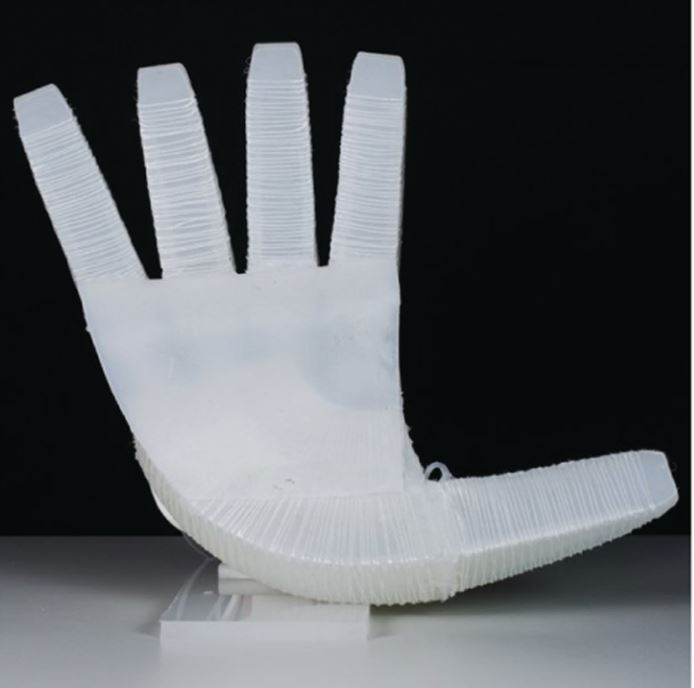
\includegraphics[height=40mm]{Images/rbo_hand2.jpg}}\quad
\subfigure[iRobot-Harvard-Yale]{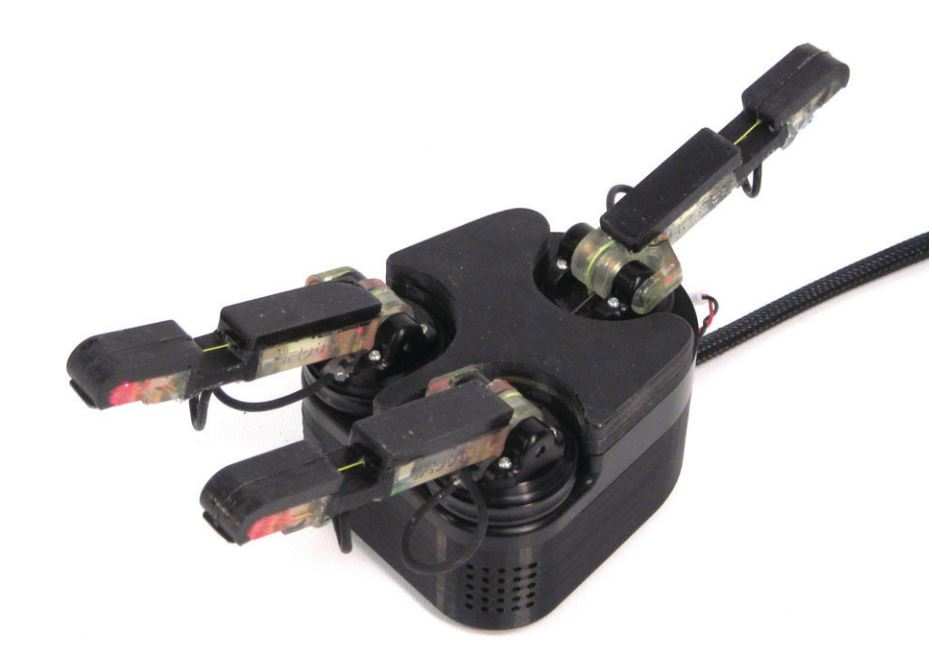
\includegraphics[height=40mm]{Images/compliant_underactuated_hand_for_robot_manipulation.jpg}}
\subfigure[Bellows fingers]{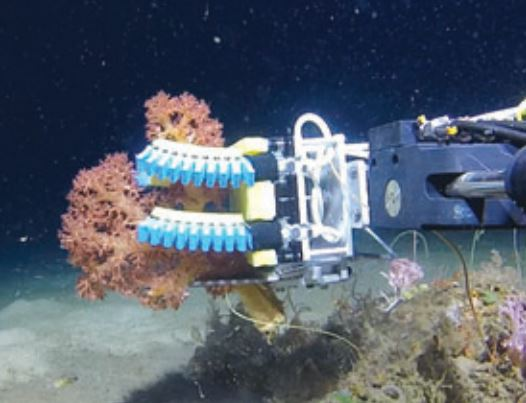
\includegraphics[height=40mm]{Images/deep_sea_hand.jpg}}
\subfigure[Soft industrial gripper from Festo AG \& Co.KG]{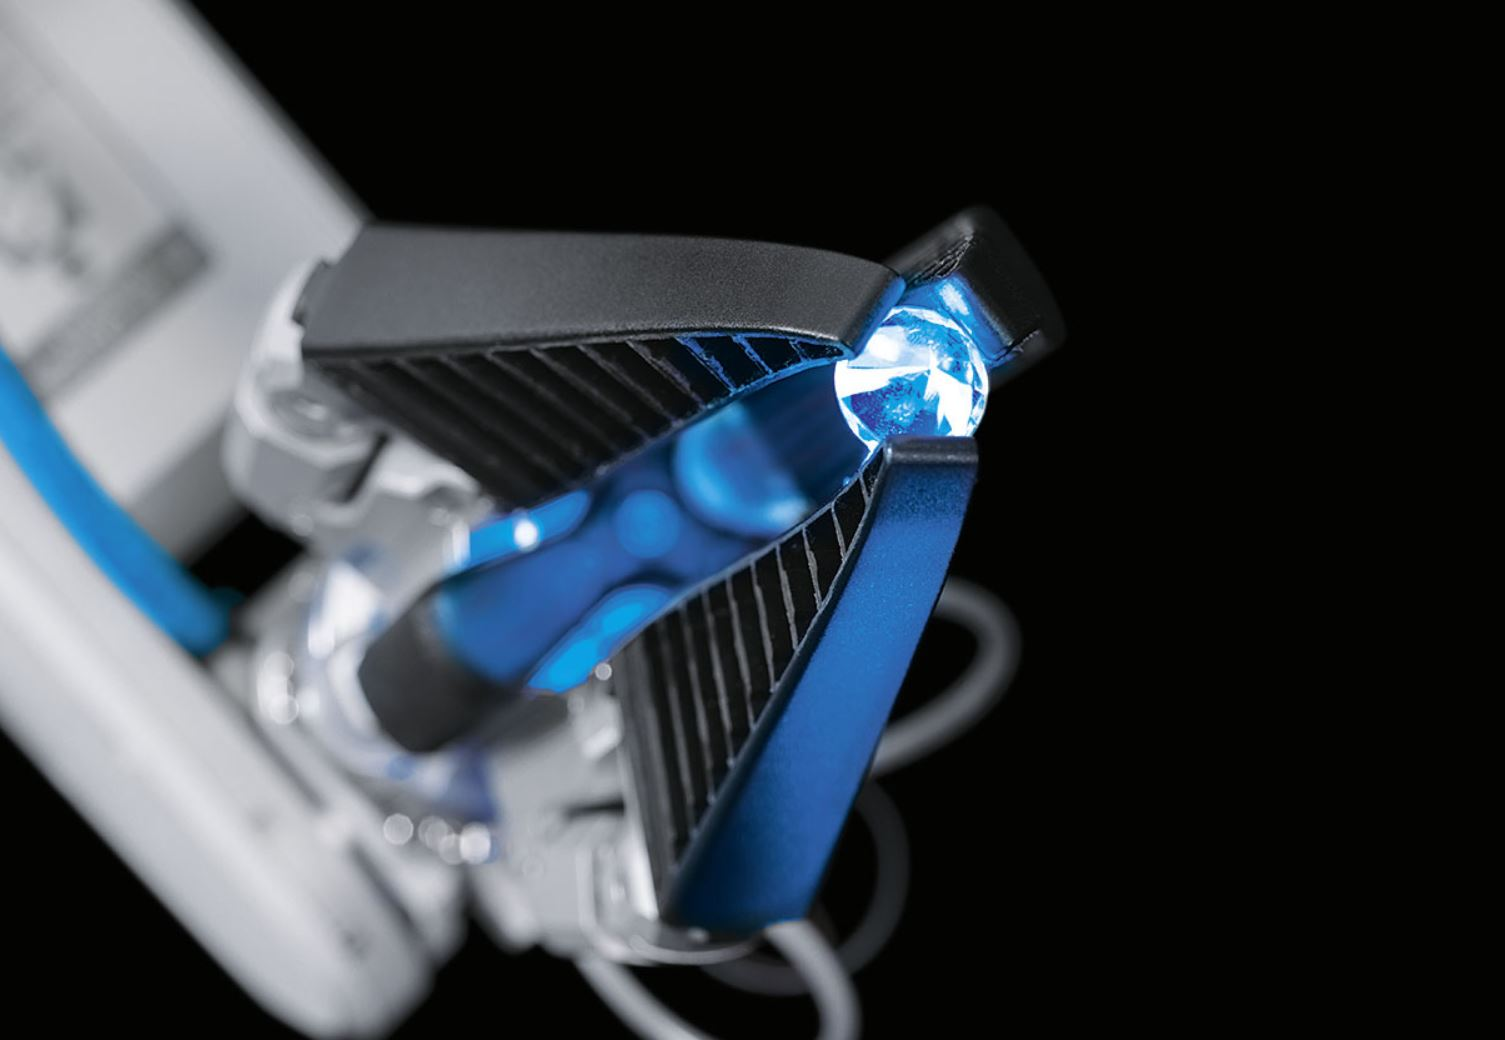
\includegraphics[height=40mm]{Images/festo.jpg}}
\caption[Robotic Hands]{\label{f:Robotic Hands} Different type of robotic hands. (a) The RBO hand is equipped with Pneuflex fingers and is actuated with pressure like the Bellows type finger for deep-sea application. (b) The iRobot-Harvard-Yale hand uses compliant joints which can also rotate.(c) Bellows fingers in deep-sea application. (d) Festo gripper with finray fingers.}
\end{figure}

\subsection{Other soft end-effectors}
\label{s:OtherSoftManipulators}

There exist other robotic grippers that are considered soft and do not take the shape of a hand with fingers placed around a palm. An example of this set up is the jamming gripper presented by Eric Brown et al. \cite{brown2010universal, amend2012positive} . It has the capability to grasp objects by changing the state in which the grains are. The transitioning between liquid-like state and solid-like state occurs through pressure changes. An obvious advantage of such a gripper is its capability to highly adapt to the morphology of the target. It also present a simplified actuation and computation compared to fingers which often are activated individually. However as simple as this solution sounds, there are a few flaws: it can have difficulties grasping objects on soft compliant surfaces.The softness of the surface  will not allow the jamming end to embrace efficiently the target as it will sunk n and not present a surface large enough for the gripper to embrace. A similar idea was developed by S. Li et al. \cite{li2017fluid} which relies also on pressure changes but instead of coffee beans uses internal origami structures. Like a muscle, it will through pressure changes, open or close. Trunk-like end-effectors are also used in grasping tasks. The bellows-type grasper from Galloway et al. \cite{galloway2016soft} is a single finger entangling itself around the target. Compared to the finger described in the same publication, it does not need a palm and can act on its own. 

There exist also several other techniques allowing a soft-touch and a seemingly gentle grasping. Some, for instance, use adhesion in a controlled way. It allows the manipulation of fragile objects since the normal force of the gripper acting on the target object can be reduced by and increase in the shear forces brought by the adhesive properties of the gripper's surface \cite{shintake2016versatile, shintake2018soft} (Figure~\ref{f:Other Effectors}). Shintake et al. \cite{shintake2018soft} distinguish two types of adhesion : electro and gecko adhesion. 

\begin{figure}[ht]
\centering
\subfigure[Jamming gripper]{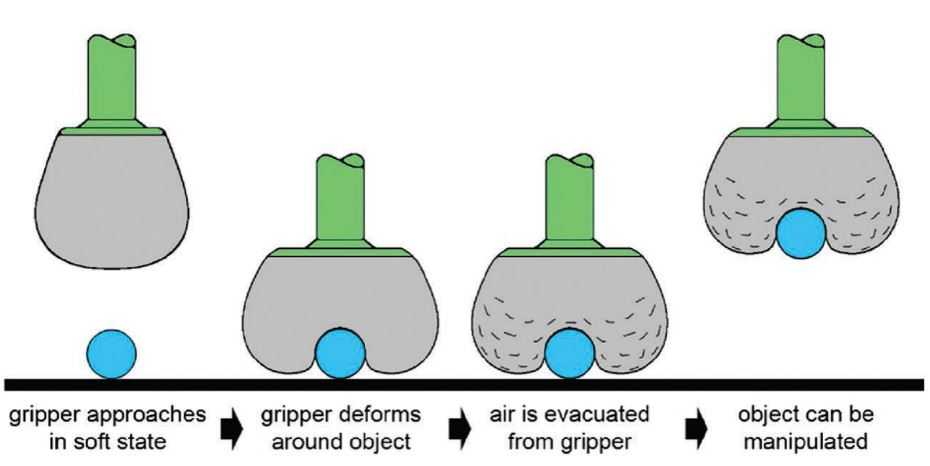
\includegraphics[height=50mm]{Images/jamming.jpg}}\quad
\subfigure[]{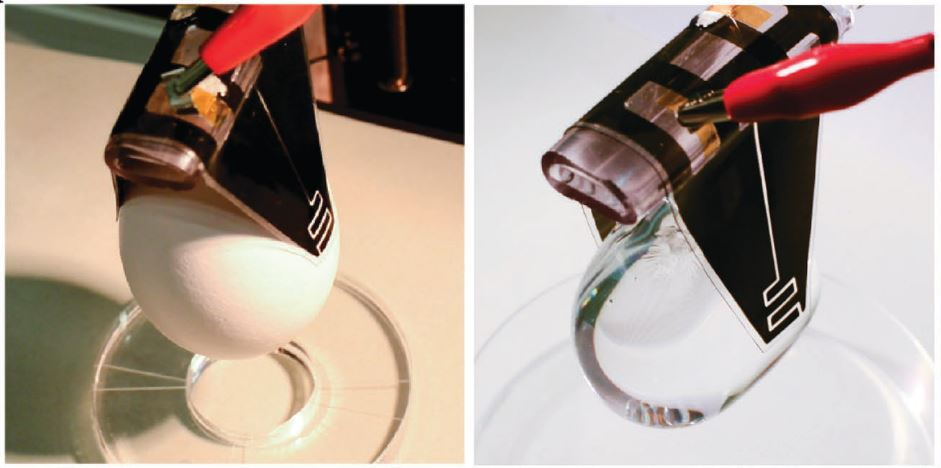
\includegraphics[height=35mm]{Images/electro_adhesion_1.jpg}}\quad
\subfigure[]{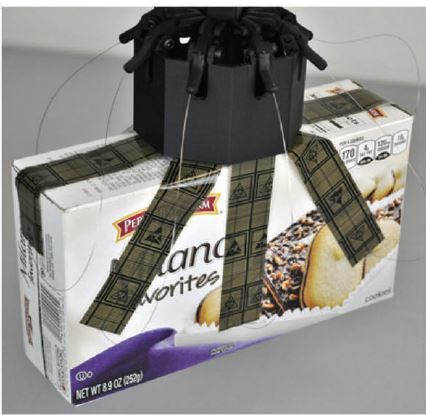
\includegraphics[height=35mm]{Images/electro_adhesion_2.jpg}}\quad
\caption[Other Effectors]{\label{f:Other Effectors} (a) The jamming of grains allows the gripper to seize target objects of various shapes. (b) Example of an electro adhesive gripper grabbing an egg and a water filled balloon.(c) Electro adhesive gripper developped by Grabit Inc.\footnote{Grabit: https://grabitinc.com/products/} }
\end{figure}

\subsection{Testing for robotic end-effectors}
\label{s:TestinginRobotics}

 Measuring the quality of a grasp is not a trivial task for soft robots. As opposed to rigid robotic hands and fingers, the sensing capabilities are restrained. Rigid links have the possibility through reacting forces and servoing to estimate accurately position and other events acting on the system. Sensors backed by accurate path planning as well as state estimation can help create a precise motion. In soft-robotics similar metrics can be applied for measuring precision.  However when it comes to measuring adaptability and gentleness, there is no unified and standardized method. It appears that testing for robotic end-effectors is disparate. Some groups use balloons with thin membranes, eggs \cite{shintake2016versatile}, tubes \cite{galloway2016soft} or other objects \cite{odhner2014compliant} suited for the task they want to achieve without generalizing and making it easy to compare with other solutions.
 
 
 Some comparisons are made with the human hand directly \cite{deimel2016novel} for example with the Kapandji test \cite{kapandji1986clinical} which records if the fingers of a hand can achieve certain positions (Figure~\ref{f:Other Testing}). This testing method could be used for comparing two five fingered robotic hands but would lack generalization to show the pros and cons of having five fingers versus two. 

 
 Nonetheless many generalization attempts have been made and are better described and summarized in a large table by Calli et al. \cite{calli2015benchmarking}. They propose with the Yale - Carnegie Mellon University - Berkeley (YCB) data set a new way to gather  solutions from around the world (Figure~\ref{f:Other Testing}). It includes different physical objects in various categories such as food items or tools. Food items can be used for example for testing some gentleness (squeezing of a fruit), whereas the tools can give an idea of the quality of a manipulation. Throughout these object sets, it becomes possible to create benchmarks and testing protocols other groups could use and try to repeat with their own gripper or manipulator. The platform is open source and promotes collaboration.
 \begin{figure}[ht]
\centering
\subfigure[]{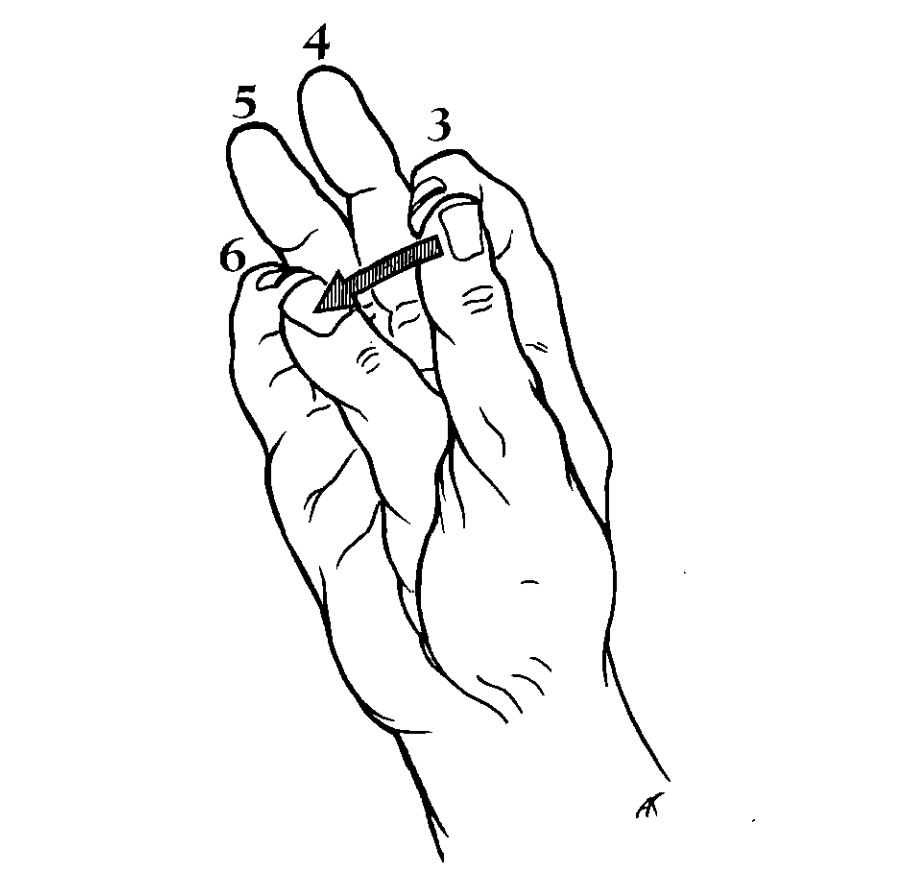
\includegraphics[height=40mm]{Images/kapandji_test.jpg}}\quad
%\subfigure[]{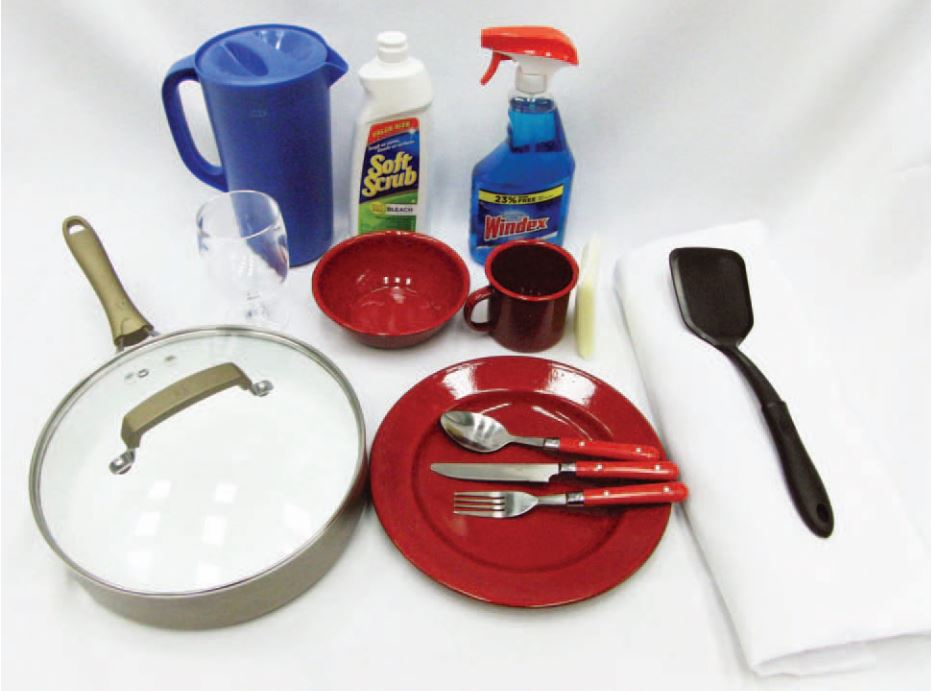
\includegraphics[height=40mm]{Images/ycb_kitchen.jpg}}\quad
\subfigure[]{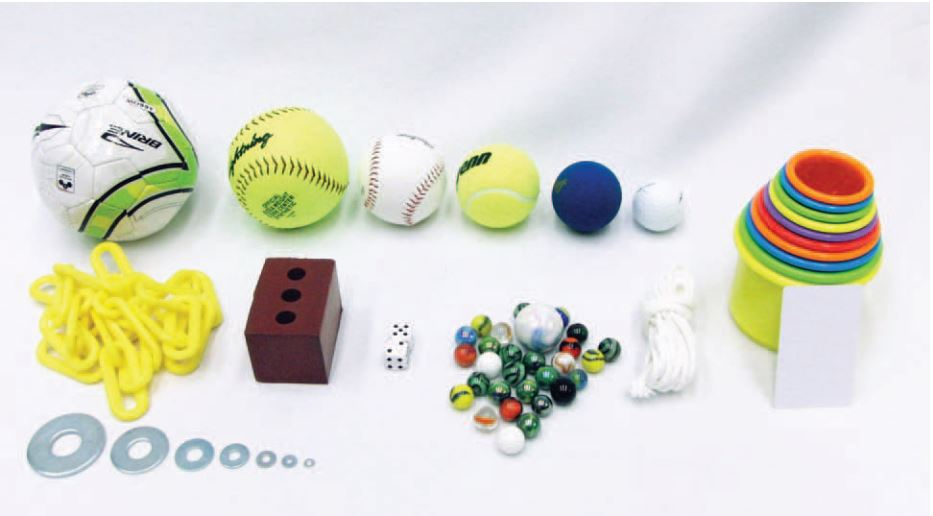
\includegraphics[height=40mm]{Images/ycb_shape.jpg}}\quad
%\subfigure[]{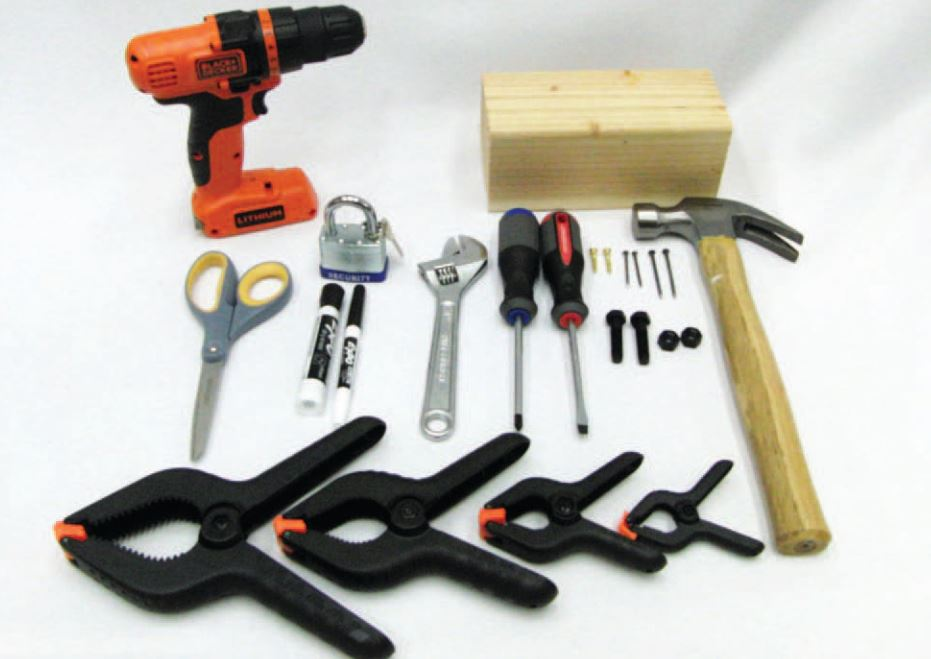
\includegraphics[height=40mm]{Images/ycb_tools.jpg}}\quad
%\subfigure[]{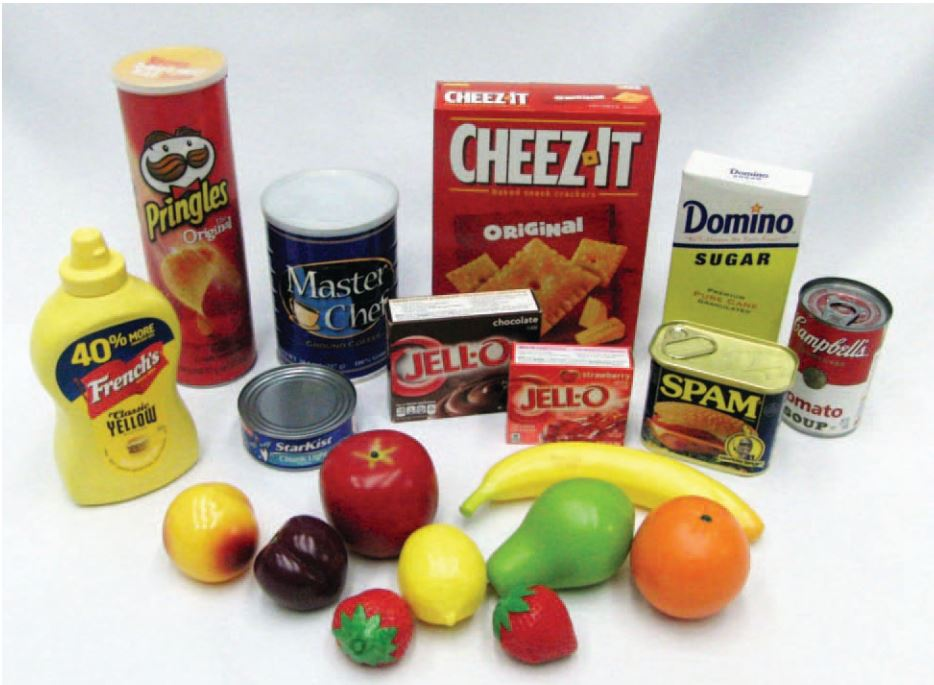
\includegraphics[height=40mm]{Images/ycb_food.jpg}}\quad
\caption[Other Testing]{\label{f:Other Testing} (a) Sketch of the opposing thumb test: In this particular test the thumb has to reach all the finger tips going from 3 to 6.(b) Extract of the YCB data-set with objects of different shapes.}
\end{figure}














\section{Methods}
\label{s:Methods}

The fingers will have bellows. Bellows arranged in a non symmetrical way along the longitudinal axis, fill themselves with pressurized air or water to simultaneously swell. The swelling bellows push each other and bend the finger.
The attempted fabrication method to achieve the desired design with an active stiffening part as well as out of plane bending will mainly rely on molding. Thanks to the CAD design tool Fusion360, molds for soft cores and soft shell will be conceived. The technique has been used in the Microrobotics Laboratory and has shown some convincing field results \cite{galloway2016soft}. The shells and cores are made out of silicone and can be poured in 3D printed molds. The inner channels of the fingers are created through embedding a soft core that would later be pulled out.

\subsection{Design}
\label{s:Design}

\subsection{Mold fabrication}
\label{s:Mold fabrication}

\subsection{Silicone properties}
\label{s: Silicone properties}

\subsection{Molding and mounting}
\label{s: Molding and mounting}







\section{Tests}
\label{s:Tests}

Testing with the gantry: what has been done to enhance its capabilities: (the vision part)

-Present the water gantry and its automated structure
How did we test?

-Test with the testing method of Clark and the protocols

-\cite{galloway2016soft}
Use the instron test to pull a tube away form the rigid-state fingers. And compare with the result presented in the Galloway paper of 2016.


\section{Summary and Contributions}
\label{s:SummaryAndContributions}

Summarize the presented work and demonstrate its contributions to the
research field or institute.



\subsection{Future Work}
\label{s:FutureWork}

Possible ways to extend the work.


% Bibliography
\newpage
\addtocontents{toc}{\vspace{.5\baselineskip}}
\addcontentsline{toc}{section}{\protect\numberline{}{References}}
\bibliography{thesis}


% Appendices (if needed)
\addtocontents{toc}{\vspace{.5\baselineskip}}
\appendix
\section{Extra Stuff}
\label{s:ExtraStuff}

Additional material such as long mathematical derivations.

\section{Miscellaneous}
\label{s:Miscellaneous}

Mention here some side quests:
the water-tank improvement
bending detector

\section{Examples}
\label{s:Examples}

This appendix provides some additional hints and examples for the
layout and style of the thesis. It is worthwhile to look at the source
file \verb|Examples.tex| for this appendix to understand how it was
created.



\subsection{Tables}

Tables are left justified and the caption appears on top as seen in
Table~\ref{t:Translations}.

\begin{table}[ht]
\caption[Translations]{\label{t:Translations}Translations.}
\begin{tabular}{ll}
\hline
\textbf{English} & \textbf{German}\\
\hline
cell phone       & Handy\\
Diet Coke        & Coca Cola light\\
\hline
\end{tabular}
\end{table}



\subsection{Figures}

Figure~\ref{f:IRISlogo} shows a simple figure with a single picture
and Figure~\ref{f:SubfigureExample} shows a more complex figure
containing subfigures.

\begin{figure}[ht]
\centering

\includegraphics[width=.6\linewidth]{Logos/IRISlogo}
\caption[IRIS logo]{\label{f:IRISlogo}IRIS logo.}
\end{figure}

\begin{figure}[ht]
\centering
\subfigure[ETH logo]{
\includegraphics[height=12mm]{Logos/ETHlogo}}\quad
\subfigure[IRIS logo]{
\includegraphics[height=12mm]{Logos/IRISlogo}}
\caption[Subfigure example]{\label{f:SubfigureExample}Two pictures as
  part of a single figure through the magic of the subfigure package.}
\end{figure}



\subsection{Units}

The SIUnits package provides nice spacing for units as demonstrated in
Table~\ref{t:SIUnits}. Use of the package also makes it easy to change
the style or even the unit text in the future.

\begin{table}[ht]
\caption[Spacing for units]{\label{t:SIUnits}Spacing for units.}
\begin{tabular}{ll}
\hline
\textbf{Output}   & \textbf{Command}\\
\hline
42m               & \verb|42m|\\
\unit{42}{\metre} & \verb|\unit{42}{\metre}|\\
42 m              & \verb|42 m|\\
\hline
\end{tabular}
\end{table}



\subsection{Miscellany}

\begin{description}

\item[Capitalization.] When referring to a named table (such as in the
  previous section), the word \emph{table} is capitalized. The same is
  true for figures, chapters and sections.

\item[Naming of structural elements.] Refer to a \verb|\section| in
  \LaTeX\ as a chapter and call a \verb|\subsection| section. (I don't
  like the way \verb|\chapter|s are rendered in the report document
  class. Hence the suboptimal markup/naming correspondence.)

\item[Bibliography.] Use \verb|bibtex| to make your life easier and to
  produce consistently formatted entries.

\item[Contractions.] Avoid contractions. For instance, use ``do not''
  rather than ``don't.''

\item[Captions.] A brief version of a caption can be provided for the
  list of figures and tables as demonstrated with the caption of
  Figure~\ref{f:SubfigureExample}. The mechanism can also be used to
  get rid of the final period of a caption in the lists.

\end{description}

\section{Journal}
\label{s:Journal}

This section Includes a day-to- day journal about the work done at Harvard. Serves as a track for experiments their results and other achievements and goal specifications.


\subsection{08/10/18}

First day at the lab meeting the team. Setting up the desktop ad different repositories. 

Getting into the code and core of the subject.

Setting up goals for the thesis. 




% Epilogue (optional)
\addtocontents{toc}{\vspace{.5\baselineskip}}
\addcontentsline{toc}{section}{\protect\numberline{}{Epilogue}}
\markright{Epilogue}
\section*{Epilogue}
\label{s:Epilogue}

Final words.



\end{document}
